% This is based on the LLNCS.DEM the demonstration file of
% the LaTeX macro package from Springer-Verlag
% for Lecture Notes in Computer Science,
% version 2.4 for LaTeX2e as of 16. April 2010
%
% See http://www.springer.com/computer/lncs/lncs+authors?SGWID=0-40209-0-0-0
% for the full guidelines.
%
% ---------------------------------------------------
% Gabarit modifié par Netkompt - 2017
% Ajouts : langue et paquets pour logiciens.
% ---------------------------------------------------

\documentclass{llncs}
\usepackage{forest}
\usepackage{prooftrees}
\usepackage[ND,SEQ]{prftree}
\usepackage{fitch}
\usepackage{cmll}
\usepackage[T1]{fontenc}
\usepackage[utf8]{inputenc}
\usepackage[french]{babel}
\def\frenchtablename{Tableau}
\usepackage{natbib}
\usepackage{fancyhdr}
\usepackage{amsmath}
\usepackage{algorithm}
\usepackage[noend]{algpseudocode}

\makeatletter
\def\BState{\State\hskip-\ALG@thistlm}
\makeatother
\pagestyle{fancy}
\fancyhf{}
\rhead{Particle Filter}
\lhead{CV Club}
\rfoot{Page \thepage}

\begin{document}

\title{Particle Filtering}
%
\author{Ajith Kemisetti\inst{}}
%

\institute{TJ CV Club\\
\email{tjcomputervision@gmail.com} \\ Site Web : 
\texttt{https://tjcompvision.github.io/}}

\maketitle              % typeset the title of the contribution

%



\section{Point Motion}
Particle filtering is an algorithm for tracking the motion of an object. Before delving into the details, the first two sections of this lecture will be dedicated to describing the problem we are trying to tackle and characteristics of this problem that complicate the solution.  
\newline
\begin{wrapfigure}{}{}
  \begin{center}
    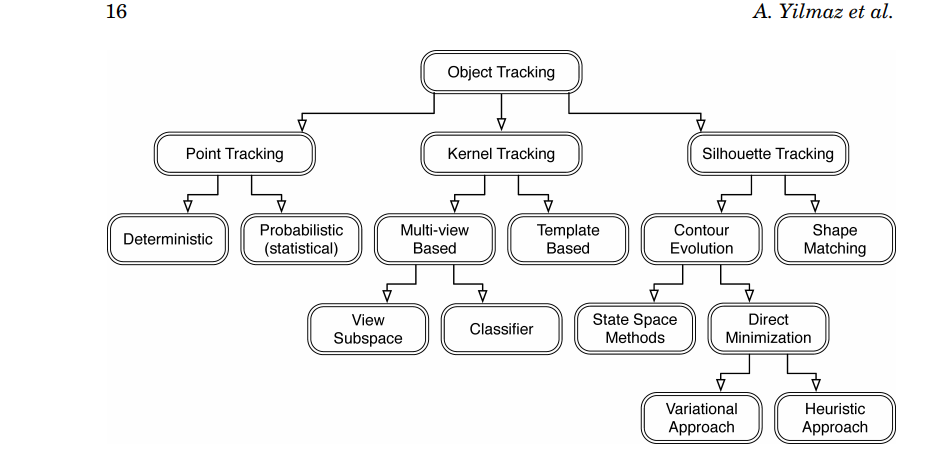
\includegraphics[width=0.8\textwidth]{Capture.PNG}
  \end{center}
  \caption{Current object tracking methodologies}
\end{wrapfigure}
\newline
\newline
\indent This section exists to provide context on current approaches to tracking individual points throughout the frames of the video. As you can see in the graphic above, there are two other approaches other than looking at points. However, this lecture will focus on the specific subset of approaches that involve treating the object as a set of points. \pagebreak
\section{Problem Description}
There are various assumptions that other methods for tracking an object try to make and it is important that, now that we've understood the general problem and modern approaches towards solving it, we have a clear understanding of the problem we are trying to analyze. Below is a list of characteristics that greatly complicate what we're trying to do.
\begin{enumerate}\bfseries
\item Multimodal: tracking 0 or more objects
\item Nonlinearity: the object won't move in a line. Rather, it will move in any sort of path, differentiable or non-differentiable
\item Noise: other objects will be moving in the background making it easy for the computer to be distracted and track the background as opposed to the intended objects.
\end{enumerate}


\section{Particle Filter Algorithm}
%
The central idea of the Particle Filter involves generating large sets of particles and intelligently predicting where the system will move. 
\newline
\newline
\indent The particle filter attempts to "approximate" the location of any object using a genetic algorithm. At its core, the algorithm involves guessing the location of the object to be everywhere at first but gaining strength based on observation to make a more reasonable guess. There is pseudocode is below.
\begin{wrapfigure}{}{}
  \begin{center}
    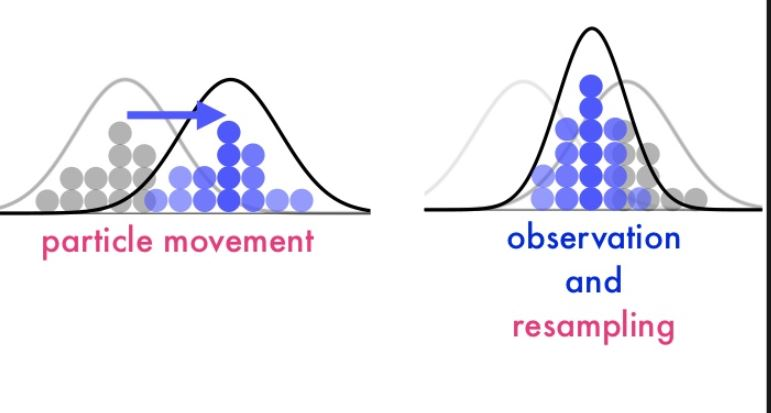
\includegraphics[width=0.8\textwidth]{pftrack.jpg}
  \end{center}
  \caption{Probability distribution}
\end{wrapfigure}
\pagebreak
\begin{algorithm}
\caption{Particle Filter}\label{euclid}
\begin{algorithmic}[1]
\Procedure{create uniform particles}{}
\State Initialize thousands of uniformly distributed particles 
\State For \textbf{N} particles, assign each particle weight/confidence \textbf{1/N} 
\State i = 0
\State MAXITER = 40
\BState \emph{top}:
\If {i >= MAXITER} \Return 
\EndIf
\BState \emph{loop}:
\State receive input and move particles with noise added
\State update weights
\State re-sample as necessary while adding in noise
\State $i \gets i+1$.
\State \textbf{goto} \emph{top}.
\EndProcedure
\end{algorithmic}
\end{algorithm}
\newline
\newline
\indent In general, each individual particle holds, at a minimum, three points of information: x and y position, and individual probability. However, velocity is also an extremely common point
of information that particles generally store. The noise added in the prediction step is to model uncertainty in real world scenarios. While the intention may have been for the object to turn 90 degrees and move a certain distance, the lack of precision in degrees rotated and in distance traveled is inevitable and must be accounted for somehow. 
\newline 
\begin{wrapfigure}{}{}
  \begin{center}
    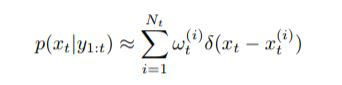
\includegraphics[width=0.4\textwidth]{filtereq1.jpg}
  \end{center}
\newline 
\indent \indent 
\textbf{N} is the number of particles, and omega is the weight of that particle at the specific time. The approximation is centered around x(t). The update weights step involves a direct implementation of Bayes' theorem. Each particle has a weight and implementing this formula will increase the weights of particles with stronger probabilities and enable much more effective tracking.
\begin{wrapfigure}{}{}
  \begin{center}
    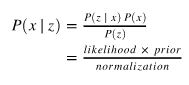
\includegraphics[width=0.4\textwidth]{bayes.jpg}
  \end{center}
\end{wrapfigure}
\newline 
\pagebreak
\indent \indent Finally, we have the re-sampling step which involves discarding particles that have weights that are far too negligible to be considered. However, simply discarding these particles will lead to a very common problem with these types of filters called the \textit{degeneracy problem}. This problem arises when you are discarding too many particles because of their low weights and are left with 3 or 4 particles which isn't a high enough number of particles to accurately represent anything. Instead the formula below is often used to compute the amount of "meaningless" particles. If this number crosses a certain threshold, re-sampling will be done. Furthermore, rather than just discard, re-sampling will involve replacing the low weight particles with high weight particles but adding some noise so they don't overlap.
\end{wrapfigure}
\begin{wrapfigure}{}{}
  \begin{center}
    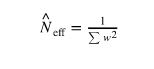
\includegraphics[width=0.3\textwidth]{sir.jpg}
  \end{center}
\end{wrapfigure}
\end{document}
